% !TEX program = xelatex
% 澳門記憶 macaumemory · 技術發展歷程
% 編譯：cd docs && xelatex -interaction=nonstopmode tech-evolution.tex（跑兩次）
\documentclass[11pt,a4paper,fontset=windows]{ctexart}

\usepackage[margin=2.1cm]{geometry}
\usepackage{amsmath,amssymb}
\usepackage{booktabs}
\usepackage{longtable}
\usepackage{array}
\usepackage{multirow}
\usepackage{xcolor}
\usepackage{graphicx}
\usepackage{float}
\usepackage{enumitem}
\usepackage{caption}
\usepackage{fancyhdr}
\usepackage{tikz}
\usetikzlibrary{arrows.meta,positioning,fit,backgrounds}
\usepackage[colorlinks=true,linkcolor=blue!55!black,urlcolor=teal!70!black]{hyperref}

\definecolor{ink}{HTML}{10243A}
\definecolor{gold}{HTML}{C8A24A}
\definecolor{teal2}{HTML}{2A7F8F}
\definecolor{red2}{HTML}{C0392B}
\definecolor{paper}{HTML}{F7F5F0}

\captionsetup{font=small,labelfont={bf,color=ink},skip=6pt}
\pagestyle{fancy}
\fancyhf{}
\fancyhead[L]{\small\color{ink}澳門記憶 macaumemory}
\fancyhead[R]{\small\color{ink}技術發展歷程}
\fancyfoot[C]{\small\thepage}
\renewcommand{\headrulewidth}{0.4pt}
\setlength{\parskip}{2pt}

\title{\vspace{-1.1cm}\textbf{\Large 從 CLIP 零樣本到多層驗證：\\[0.15cm]
城市記憶系統的技術發展歷程}\\[0.35cm]
\large Technology Evolution of an Urban Memory System:\\[0.1cm]
\large From Zero-Shot CLIP to a Multi-Stage Verification Pipeline\\[0.4cm]
\normalsize 技術歷程報告}
\author{}
\date{\today}

\begin{document}
\maketitle
\thispagestyle{fancy}

\begin{abstract}
\noindent
本報告記錄「城市記憶系統」在八個階段中的技術演進：從最初的 CLIP 零樣本影像嵌入，到加入地理先驗、自訓 YOLO 建築偵測器、資料與標註的反覆清洗、視覺語言模型（VLM）介入品管、編碼器更替為 DINOv2、加入局部特徵幾何驗證，最後以 VLM 標註訓練線性探針分類器。每一階段都列出\textbf{動機、方法、量化結果、以及被推翻的假設}。核心量化結論：跨條件重辨識 AUC 由 0.850 提升至 \textbf{0.993}；真實照片的同棟／不同棟判別間距由 0.138 擴大到 \textbf{0.275}；幾何驗證可在「內點 $\ge$ 15」時達到 \textbf{100\% 精確率}；獨立實拍分類準確率由零樣本的 53.5\% 提升至 \textbf{67.0\%}（訓練分布內 80.4\%）。同時，本報告如實記錄了三個失敗或誤判：把分布外輸入當成方法缺陷、內部驗證集因資料洩漏而不可比、以及 DISK+LightGlue 的整合失敗。
\end{abstract}

\vspace{0.2cm}
\noindent\textbf{關鍵詞：} 視覺場所重辨識（VPR）、CLIP、DINOv2、SALAD、幾何驗證、RANSAC、視覺語言模型、自訓練、YOLO、資料洩漏

\newpage
\tableofcontents
\newpage

% ============================================================
\section{技術時間線總覽}

\begin{figure}[H]
\centering
\begin{tikzpicture}[scale=0.9, transform shape, font=\small,
  st/.style={draw=ink!40, fill=paper, rounded corners, inner sep=5pt, text width=2.5cm, align=center, minimum height=1.5cm},
  hot/.style={draw=teal2, fill=teal2!12, line width=1pt, rounded corners, inner sep=5pt, text width=2.5cm, align=center, minimum height=1.5cm},
  win/.style={draw=gold, fill=gold!16, line width=1.2pt, rounded corners, inner sep=5pt, text width=2.5cm, align=center, minimum height=1.5cm}]
\node[hot] (s1) at (0,0) {\textbf{階段 1}\\CLIP 零樣本\\AUC 0.950};
\node[hot] (s2) at (3.1,0) {\textbf{階段 2}\\地理先驗\\90 m 候選};
\node[hot] (s3) at (6.2,0) {\textbf{階段 3}\\自訓 YOLO\\mAP50 0.594};
\node[hot] (s4) at (9.3,0) {\textbf{階段 4}\\資料與標註迭代\\獨立驗收 65\%};
\node[win] (s5) at (12.4,0) {\textbf{階段 5}\\VLM 品管\\找出 19\% 錯誤};
\node[win] (s6) at (0,-2.6) {\textbf{階段 6}\\編碼器換 DINOv2\\E2 +0.143};
\node[win] (s7) at (3.1,-2.6) {\textbf{階段 7}\\幾何驗證\\內點 ≥15 零誤判};
\node[win] (s8) at (6.2,-2.6) {\textbf{階段 8}\\VLM 標註＋探針\\分類 67.0\%};
\node[draw=red2!50, fill=red2!8, rounded corners, inner sep=5pt, text width=5.6cm, align=center] (todo) at (10.6,-2.6)
  {下一階段：主動學習閉環\\＋ OOOSplat 真實多視角資料};
\draw[-{Latex[length=2mm]}] (s1)--(s2); \draw[-{Latex[length=2mm]}] (s2)--(s3);
\draw[-{Latex[length=2mm]}] (s3)--(s4); \draw[-{Latex[length=2mm]}] (s4)--(s5);
\draw[-{Latex[length=2mm]}] (s5.south) -- (12.4,-1.3) -- (0.2,-1.3) -- (s6.north);
\draw[-{Latex[length=2mm]}] (s6)--(s7); \draw[-{Latex[length=2mm]}] (s7)--(s8);
\draw[-{Latex[length=2mm]}, dashed] (s8)--(todo);
\end{tikzpicture}
\caption{八個技術階段。藍綠色為「建立能力」，金色為「提升精度與可信度」。}
\end{figure}

\begin{table}[H]
\centering\small
\begin{longtable}{@{}p{1.5cm}p{4.6cm}p{5.6cm}p{4.2cm}@{}}
\toprule
\textbf{階段} & \textbf{做了什麼} & \textbf{為什麼} & \textbf{量化結果} \\
\midrule
1 & CLIP 零樣本影像嵌入重辨識 & 無需標註即可判斷「是否同一棟」 & 受控 AUC 0.950；實拍 0.796 \\
2 & 加入 90 m 地理先驗 & 視覺無法區分外觀相近的不同建築 & 路氹城誤判全部排除 \\
3 & 自訓 11 類建築偵測器 & COCO 80 類中沒有「建築」 & mAP50 0.594（舊驗證集） \\
4 & 資料擴增與標註清洗 & 弱標註與樣本不足是精度瓶頸 & 獨立驗收偵測 57\%$\to$65\% \\
5 & DeepSeek 視覺模型品管 & 本地模型無法發現自己的偏誤 & 568 張中 19\% 標註需修正 \\
6 & CLIP $\to$ DINOv2 & CLIP 是圖文對比訓練，不利細粒度個體辨識 & E2 0.850$\to$0.993 \\
7 & SIFT + RANSAC 幾何驗證 & 為「無 GPS」情境提供第二道防線 & 內點 $\ge$15 時精確率 100\% \\
8 & VLM 標註 + 線性探針 & 零樣本分類只有 53.5\% & 獨立實拍 67.0\%（+13.5 點） \\
\bottomrule
\end{longtable}
\caption{八個階段的動機與結果一覽。}
\end{table}

% ============================================================
\section{階段 1：CLIP 零樣本重辨識}

\subsection{動機}
一開始的目標是「判斷兩張照片是否為同一棟建築」，但沒有任何標註資料，也不可能為每棟建築收集訓練集。CLIP 的零樣本能力（以文字提示詞分類、以影像嵌入比對）看起來是最低成本的起點：512 維影像向量、餘弦相似度、無需訓練。

\subsection{方法}
\begin{enumerate}[leftmargin=1.4em,itemsep=1pt]
  \item 以 CLIP ViT-B/32 產生 512 維 L2 正規化影像嵌入；
  \item 相似度即餘弦內積；
  \item 正樣本＝同一棟建築的不同視角／不同拍攝者；負樣本＝不同建築；
  \item 以 AUC（Mann-Whitney U 統計量）評估，並掃描閾值求 TPR/FPR。
\end{enumerate}

\subsection{結果}
\begin{table}[H]
\centering\small
\begin{tabular}{@{}lrrrr@{}}
\toprule
\textbf{實驗} & \textbf{正樣本} & \textbf{負樣本} & \textbf{AUC} & \textbf{同棟／不同棟均值} \\
\midrule
E1 受控多視角渲染 & 330 & 1{,}440 & 0.950 & $0.901\pm0.036$ / $0.758\pm0.073$ \\
E1b 文物 & 132 & 144 & 0.998 & — \\
E1r 真實照片 & 205 & 4{,}845 & \textbf{0.796} & $0.716\pm0.136$ / $0.578\pm0.093$ \\
\bottomrule
\end{tabular}
\caption{CLIP 世代的基準結果。受控條件表現良好，真實照片明顯下滑。}
\end{table}

\subsection{暴露的三個問題}
\begin{enumerate}[leftmargin=1.4em,itemsep=2pt]
  \item \textbf{相似建築會互相誤判}：負樣本中，澳門倫敦人與澳門銀河的平均相似度達 0.874，誤判率 72.2\%。
  \item \textbf{閾值不可遷移}：在渲染圖上 0.86 可認出 86.1\% 的同棟，套到真實照片只剩 14.1\%。
  \item \textbf{分類能力被誤判}：最初以 3D 渲染圖測得「CLIP 分類只有 3.0\%」，一度以為 CLIP 不能用於建築分類；補上真實照片集後發現實拍可達 53.5\%——\textbf{原結論是分布外輸入造成的假象}。
\end{enumerate}

% ============================================================
\section{階段 2：地理先驗的引入}

\subsection{誤判來源分析}
把所有負樣本按建築配對拆開，逐對計算誤判率：

\begin{table}[H]
\centering\small
\begin{tabular}{@{}lrr@{}}
\toprule
\textbf{建築配對} & \textbf{平均相似度} & \textbf{相似度 $>0.86$ 的比例} \\
\midrule
澳門倫敦人 vs 澳門銀河 & 0.874 & \textbf{72.2\%} \\
澳門巴黎人 vs 澳門銀河 & 0.840 & 31.2\% \\
澳門倫敦人 vs 澳門巴黎人 & 0.826 & 18.8\% \\
其餘 7 組配對 & 0.70--0.75 & \textbf{0.0\%} \\
\bottomrule
\end{tabular}
\caption{視覺誤判 100\% 集中在路氹城三棟外觀相近的度假村。}
\end{table}

\noindent 關鍵事實：這三棟建築兩兩相距 \textbf{至少 296 公尺}（中位數 4{,}302 公尺）。以 90 公尺為半徑的地理先驗，可直接排除全部誤判候選。

\subsection{架構轉變}
\begin{quote}
\textbf{視覺比對只負責「同一棟的不同角度」；地理先驗負責「不可能是我」。}
\end{quote}

\noindent 這個分工成為後續所有設計的基礎：視覺模型不需要（也不可能）做到完美，只要在「地理上可能的候選」中做出判斷即可。

% ============================================================
\section{階段 3：為什麼要自己訓練 YOLO}

\subsection{動機}
COCO 預訓練的 YOLO \textbf{沒有「建築」這個類別}（80 類中最接近的是「房屋」概念的缺失）。要偵測建築，必須自建資料集並微調。

\subsection{如何訓練 YOLO：五步資料管線}
\begin{enumerate}[leftmargin=1.4em,itemsep=2pt]
  \item \textbf{抓圖}：以 Wikimedia Commons 的\textbf{人工策展分類}（如 \texttt{Category:Churches in Macau}）為主、全文檢索為輔，並遞迴走訪子分類；以 SHA1 去重避免同一張圖重複進入資料集。
  \item \textbf{CLIP 自動清洗}：三道關卡——類別關（CLIP 12 類機率）、雜物關（與「食物／招牌／人像／文件」等提示詞的相對相似度）、室內關（室內照對偵測器是雜訊）。清洗後保留約 44\%。
  \item \textbf{自動預標註}：以 YOLO-World 開放詞彙偵測「建築在哪」，\textbf{類別直接採用資料夾標籤}，因此人工只需修正框、不需重新分類。
  \item \textbf{防洩漏＋分層切分}：以「檔名建築鍵 ＋ CLIP 相似度」雙重分組，確保同一棟建築不會同時出現在訓練與驗證集；再按類別分層，保證每個類別在驗證集都有代表。
  \item \textbf{訓練}：YOLO11n、100 epochs、640 px、batch 16。
\end{enumerate}

\subsection{第一版結果與三個教訓}
\begin{table}[H]
\centering\small
\begin{tabular}{@{}lrrl@{}}
\toprule
\textbf{類別} & \textbf{訓練張數} & \textbf{AP50} & \textbf{備註} \\
\midrule
中式廟宇 temple & 37 & 0.995 & 外觀獨特 \\
葡式殖民 portuguese & 32 & 0.845 & \\
現代高層住宅 & 21 & 0.822 & \\
天主教教堂 church & 31 & 0.795 & 與騎樓唐樓易混 \\
牌坊紀念物 monument & 51 & 0.675 & \\
工業倉庫 industrial & 14 & 0.670 & 樣本過少 \\
村落民居 village & 47 & 0.650 & \\
騎樓唐樓 tong\_lau & 21 & 0.404 & \\
酒店娛樂場 casino\_hotel & 29 & 0.318 & 與高層住宅易混 \\
公共建築 civic & 29 & 0.271 & \\
街市 market & 10 & 0.089 & 樣本過少且含非建築場景 \\
\midrule
\textbf{全體} & \textbf{322} & \textbf{0.594} & mAP50-95 = 0.410 \\
\bottomrule
\end{tabular}
\caption{第一版 YOLO11n 的驗證集結果。}
\end{table}

\begin{enumerate}[leftmargin=1.4em,itemsep=2pt]
  \item \textbf{弱標註是最大瓶頸}：框由 YOLO-World 產生，位置正確但不夠緊，直接壓低 mAP50-95。
  \item \textbf{驗證集分數會高估}：另以完全獨立的照片集驗收，發現\textbf{未見過的建築偵測率僅 37\%}，與驗證集的 0.594 落差巨大。
  \item \textbf{類別極度不平衡}：村落 55 張 vs 街市 10 張，AP 相差十倍以上。
\end{enumerate}

% ============================================================
\section{階段 4：資料與標註的迭代}

\subsection{放寬類別關：救回被誤殺的圖}
第一版的「類別關」用 CLIP 的 top-1 類別做硬性判斷，但 CLIP 會把大三巴牌坊判成「教堂」——這是分類體系差異，不是資料錯誤。把類別關放寬後：

\begin{table}[H]
\centering\small
\begin{tabular}{@{}lrrr@{}}
\toprule
\textbf{類別} & \textbf{嚴格清洗} & \textbf{放寬後} & \textbf{變化} \\
\midrule
街市 market & 47 & 83 & $+36$ \\
騎樓唐樓 tong\_lau & 35 & 78 & $+43$ \\
工業倉庫 industrial & 30 & 64 & $+34$ \\
公共建築 civic & 41 & 80 & $+39$ \\
天主教教堂 church & 36 & 61 & $+25$ \\
\midrule
\textbf{總計} & \textbf{496} & \textbf{727} & $\mathbf{+231}$ \\
\bottomrule
\end{tabular}
\caption{放寬類別關後救回 231 張，正好補上最缺乏的類別。}
\end{table}

\subsection{用已訓練模型反向清洗}
抽樣目視後發現放寬的代價：\texttt{church} 資料夾裡出現現代高樓、\texttt{tong\_lau} 裡出現度假村。因此以「在乾淨子集上訓練出來的模型」當裁判，把「模型強烈認為不是這個類別」（信心 $\ge 0.55$）的圖移到 \texttt{images/suspect/}：

\begin{itemize}[leftmargin=1.4em,itemsep=1pt]
  \item 727 張中，模型同意 435、模型沒偵測到 200、\textbf{強烈不同意 62}（8.5\%）；
  \item 流向合理：\texttt{tong\_lau}$\to$度假村 6 張、$\to$高層住宅 5 張。
  \item 最終可用資料：\textbf{665 張}（相較第一版 496 張增加 34\%）。
\end{itemize}

\subsection{自訓練補框}
以第一版模型掃描「YOLO-World 漏掉、尚未進入訓練集」的圖，能補上 \textbf{33 張}（信心 $\ge$ 0.5）。數量不多，但證明自訓練閉環可行——限制在於第一版模型本身還不夠強。

\subsection{一個被發現的真 bug}
三個品管腳本都用 \texttt{stem.split("\_")[0]} 取類別，遇到\textbf{多字類別名}（\texttt{casino\_hotel}、\texttt{tong\_lau}、\texttt{residential\_tower}）會切成 \texttt{casino}／\texttt{tong}／\texttt{residential}，導致 \textbf{130 張（23\%）被靜默跳過}。修正為「最長前綴匹配」後，覆蓋率由 438 張回到 \textbf{568 張}。

\begin{quote}
\textbf{教訓：}如果沒有檢查「腳本實際處理了幾張」，這個 bug 會讓所有品管結論只覆蓋 77\% 的資料，而漏掉的正好是三個最需要檢查的類別。
\end{quote}

\subsection{第二版訓練與公平對比}
第二版改用 \textbf{YOLO11s（943 萬參數，第一版 260 萬）}、\textbf{768 px}（第一版 640）、\textbf{451 張訓練}（第一版 322）、150 epochs＋cosine LR。

\begin{table}[H]
\centering\small
\begin{tabular}{@{}lrrr@{}}
\toprule
\textbf{評估方式} & \textbf{第一版 yolo11n} & \textbf{第二版 yolo11s} & \textbf{說明} \\
\midrule
內部驗證集 mAP50（117 張，兩者共同） & 0.691 & 0.519 & \textbf{不公平}：新驗證集部分來自舊訓練集 \\
\midrule
獨立照片：偵測率 & 57\% & \textbf{65\%} & 兩者都沒見過 \\
獨立照片：類別準確率 & 43\% & \textbf{56\%} & \\
獨立照片：訓練見過者 & 95\% / 95\% & 93\% / 92\% & 略降（不再死背） \\
\bottomrule
\end{tabular}
\caption{在同一組獨立照片上的公平對比。內部驗證集因資料洩漏而不可比。}
\end{table}

\begin{quote}
\textbf{方法論教訓：}當驗證集被重新切分後，舊模型可能「訓練時見過」新驗證集的圖，分數會被灌水（本例中 \texttt{monument} 出現 0.984 vs 0.348 這種極端差距）。\textbf{唯一可靠的比較方式是完全獨立的外部資料集。}
\end{quote}

% ============================================================
\section{階段 5：視覺語言模型介入品管}

\subsection{動機}
本地模型（CLIP 判斷、自訓 YOLO）有兩個無法自我發現的盲點：一是 CLIP 的類別偏見（大三巴＝教堂），二是自訓模型只學過現有標註，無法察覺標註本身的錯誤。需要一個\textbf{第三方裁判}。

\subsection{方法}
使用 DeepSeek 視覺模型（\texttt{deepseek-flash}，官方 API 已支援圖片輸入）：
\begin{itemize}[leftmargin=1.4em,itemsep=1pt]
  \item 每次請求送 12 張圖，要求\textbf{只輸出 JSON}（類別 ＋ 信心）；
  \item \texttt{detail: low} 將圖片壓到 512$\times$512，\textbf{每張圖僅約 238 tokens}；
  \item 結果寫入本機快取（\texttt{.cache/vlm/labels.json}），重跑不再計費；
  \item 加上「類別定義歧義表」：如 \texttt{monument}$\leftrightarrow$\texttt{church}（大三巴牌坊本身是教堂遺址）、\texttt{portuguese}$\leftrightarrow$\texttt{civic}，這類不一致不自動改標註。
\end{itemize}

\subsection{結果（568 張）}
\begin{table}[H]
\centering\small
\begin{tabular}{@{}lrrl@{}}
\toprule
\textbf{VLM 判定} & \textbf{張數} & \textbf{占比} & \textbf{處理} \\
\midrule
同意（高信心） & 288 & 50.7\% & 保留 \\
\textbf{類別定義歧義} & 93 & 16.4\% & 人工複核，不自動改 \\
\textbf{真錯誤（跨類別）} & 85 & 15.0\% & 修正標籤 \\
\textbf{不是建築物} & 23 & 4.0\% & 移出訓練集 \\
不同意（低信心）／同意（低信心） & 65 / 37 & 18.0\% & 保留 \\
\bottomrule
\end{tabular}
\caption{VLM 品管結果：合計 108 張（19\%）的標註需要修正。}
\end{table}

\subsection{人工複核抽樣}
對 13 張「高信心反對」的圖逐張目視判斷，結論：\textbf{約 10 張 VLM 是對的}，抓到的是本地模型完全無法發現的錯誤類型——
「街市」資料夾裡是市場\textbf{室內攤位}、「村落」裡是\textbf{黃色教堂}、「廟宇」裡\textbf{根本沒有建築}、「工業」裡是石牆紀念物、「公共」裡有 3 張明顯是葡式殖民建築。
其中 2 張是\textbf{類別定義歧義}（大三巴牌坊：VLM 說教堂、我們的體系歸為牌坊），正是需要人工而非自動處理的情況。

% ============================================================
\section{階段 6：編碼器世代更替（CLIP $\to$ DINOv2）}

\subsection{動機}
CLIP 是「影像—文字對比」訓練出來的，特徵偏向語意類別，對「同一棟建築的不同角度」這種細粒度個體辨識天生不利。DINOv2 是純視覺自監督，特徵保留更多實例細節，是目前視覺場所重辨識（VPR）領域的主流骨幹。

\subsection{實作要點}
\begin{itemize}[leftmargin=1.4em,itemsep=1pt]
  \item 以 \texttt{transformers} 載入 \texttt{facebook/dinov2-base}，取 CLS token 與 patch token 的 GeM 池化（$p=3$），並做水平翻轉平均；
  \item \textbf{等比縮放最短邊＋中心裁切}（保留外觀比例），而非直接壓成正方形；
  \item 特徵快取\textbf{依編碼器分檔}（\texttt{embeddings-<model>.npz}），避免換模型時誤用舊特徵。
\end{itemize}

\begin{figure}[H]
\centering
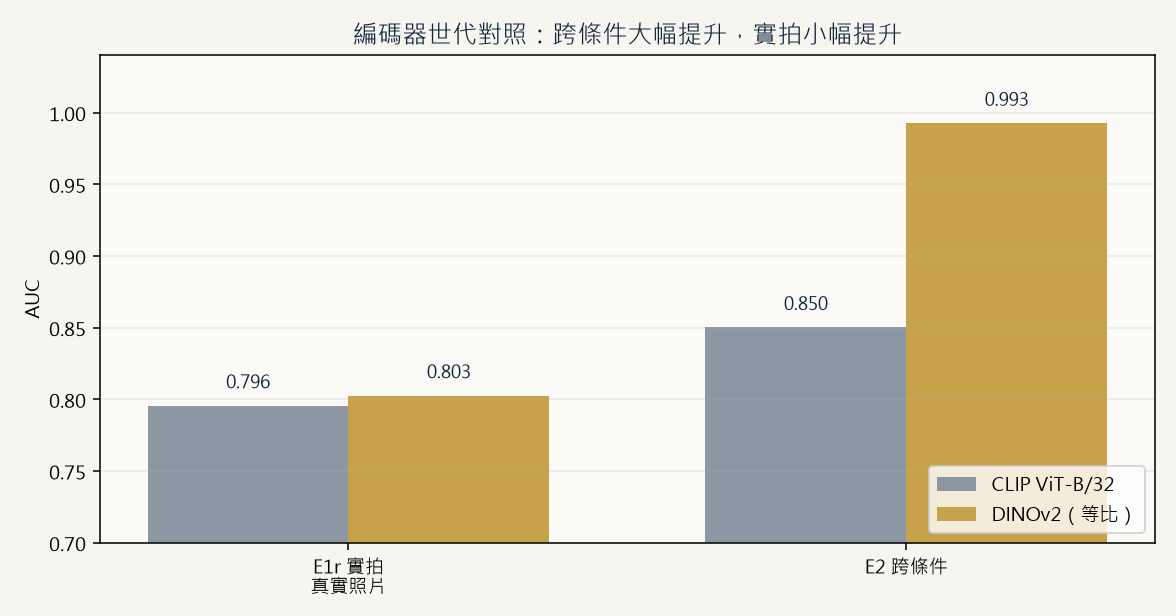
\includegraphics[width=0.86\linewidth]{figs/encoder-compare.png}
\caption{編碼器世代對照。跨條件（E2）提升最顯著，實拍（E1r）小幅提升。}
\end{figure}

\subsection{結果}
\begin{table}[H]
\centering\small
\begin{tabular}{@{}lrrrrr@{}}
\toprule
\textbf{設定} & \textbf{E1} & \textbf{E1b} & \textbf{E1r} & \textbf{E2} & \textbf{實拍最佳閾值} \\
\midrule
CLIP ViT-B/32（原基準） & 0.950 & 0.998 & 0.796 & 0.850 & 0.689 \\
DINOv2（壓成正方形） & 0.998 & 1.000 & 0.789 & 0.993 & 0.534 \\
\textbf{DINOv2（等比＋裁切）} & \textbf{0.998} & 1.000 & \textbf{0.803} & \textbf{0.993} & \textbf{0.193} \\
\bottomrule
\end{tabular}
\caption{編碼器對照。DINOv2 在受控與跨條件上大幅領先。}
\end{table}

\subsection{三個關鍵發現}
\begin{enumerate}[leftmargin=1.4em,itemsep=2pt]
  \item \textbf{判別間距翻倍}：實拍的同棟／不同棟相似度差距由 0.138 擴大到 \textbf{0.275}。間距比 AUC 更能反映「閾值穩不穩、能不能泛化到新資料」。
  \item \textbf{預處理比換模型更重要}：壓成正方形 0.789、等比縮放＋中心裁切 0.803。這個 0.014 的差距\textbf{比 CLIP 與 DINOv2 之間的差距還大}。
  \item \textbf{產品閾值必須重新校準}：CLIP 最佳閾值 0.689，DINOv2 是 \textbf{0.193}（DINOv2 餘弦值整體偏低）。原先產品使用的 0.86 對兩者都不適用。
\end{enumerate}

\noindent 附帶發現：輸入邊長 336 px 與 518 px 的結果\textbf{完全相同}，池化方式（CLS 或 CLS+GeM）與翻轉增強影響也都在 0.002 以內——因此採用 336 px 以節省算力。

% ============================================================
\section{階段 7：幾何驗證（第二道防線）}

\subsection{動機}
地理先驗能排除「外觀相近但距離很遠」的誤判，但\textbf{沒有 GPS 時就失效}（室內、地下、GPS 漂移）。幾何驗證提供不依賴位置的第二道防線：同棟不同角度會有大量\textbf{幾何一致}的特徵對應；不同棟即使整體相似，也難以找到一致的內點。

\subsection{方法}
\begin{enumerate}[leftmargin=1.4em,itemsep=1pt]
  \item 全局檢索：DINOv2 餘弦相似度取 top-1 候選（門檻 0.15）；
  \item 局部特徵：OpenCV SIFT（最多 2048 關鍵點）＋ Lowe 比率檢驗（0.75）；
  \item 幾何一致性：\texttt{cv2.findHomography} 搭配 \textbf{USAC\_MAGSAC} 穩健估計，統計內點數。
\end{enumerate}

\begin{figure}[H]
\centering
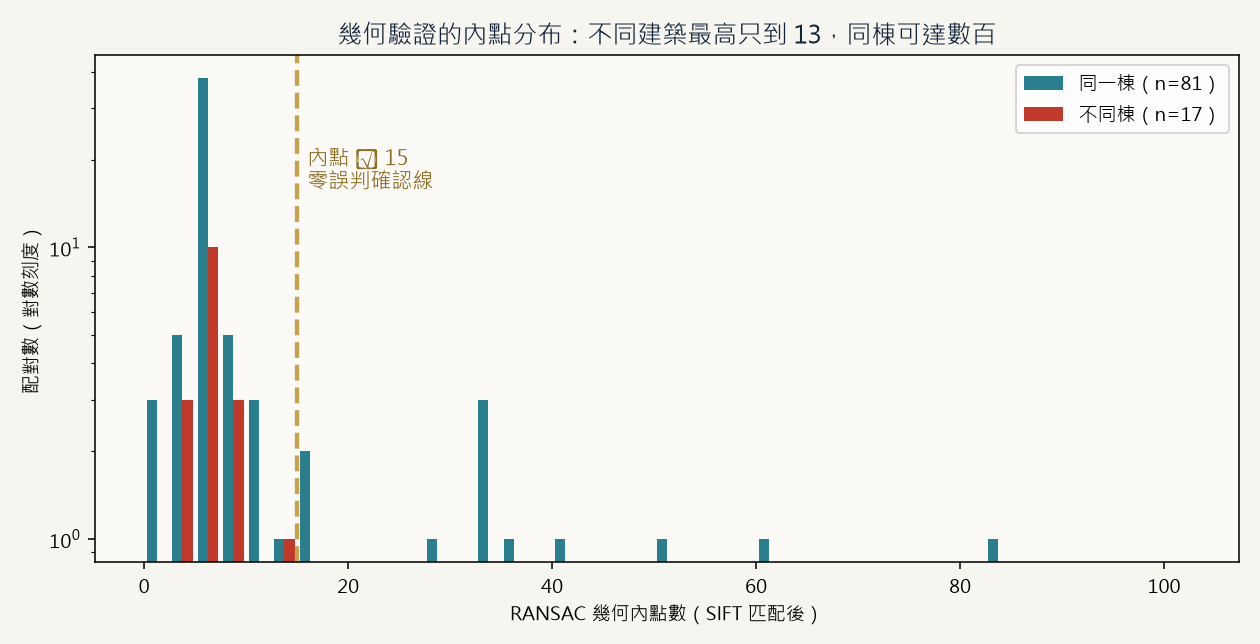
\includegraphics[width=0.82\linewidth]{figs/geo-inliers.png}
\caption{內點分布完全分離：不同建築最高只到 13 個內點，同棟可達數百。}
\end{figure}

\subsection{結果}
\begin{table}[H]
\centering\small
\begin{tabular}{@{}lrrrrr@{}}
\toprule
\textbf{組別} & \textbf{中位內點} & \textbf{p90} & \textbf{最大} & \textbf{內點為 0 的比例} \\
\midrule
同一棟建築 & 7 & \textbf{501} & 2048 & 4\% \\
不同建築 & 6 & 8 & \textbf{13} & 0\% \\
\bottomrule
\end{tabular}
\caption{內點分布：不同建築的上限只有 13，形成天然的安全邊界。}
\end{table}

\begin{table}[H]
\centering\small
\begin{tabular}{@{}lrrrr@{}}
\toprule
\textbf{內點門檻} & \textbf{接受同棟} & \textbf{接受不同棟} & \textbf{精確率} & \textbf{召回} \\
\midrule
5 & 73 & 14 & 83.9\% & 90.1\% \\
10 & 30 & 1 & 96.8\% & 37.0\% \\
15 & 26 & \textbf{0} & \textbf{100\%} & 32.1\% \\
20 & 24 & 0 & 100\% & 29.6\% \\
\bottomrule
\end{tabular}
\caption{內點門檻掃描。$\ge 15$ 時誤判為零。}
\end{table}

\subsection{定位：確認器，不是過濾器}
幾何驗證只能確認 \textbf{32\%} 的同棟配對。原因是原理性的：\textbf{若兩張照片拍的是同一棟建築的不同立面，它們之間沒有共同的視覺內容，任何幾何方法都無法確認}。因此正確的用法是：

\begin{quote}
\textbf{內點 $\ge$ 15 $\Rightarrow$ 確定同一棟（100\% 精確），可直接歸戶、不需 GPS；\\ 內點 $<$ 15 $\Rightarrow$ 退回全局相似度＋地理先驗。}
\end{quote}

\subsection{誠實記錄：一次失敗的整合}
同時嘗試了學習式特徵與匹配器（kornia 的 DISK + LightGlue，理論上比 SIFT 更耐大視角變化），但在 kornia 0.8.3 上\textbf{整合失敗}：無論是否對關鍵點座標做正規化，LightGlue 都回傳 0 個匹配（同一對圖 SIFT 可得 29 個匹配、7 個內點）。程式碼保留但預設使用 SIFT+RANSAC。\textbf{本階段的結論不依賴 LightGlue。}

% ============================================================
\section{階段 8：VLM 造標註 $\to$ 線性探針分類}

\subsection{動機}
CLIP 零樣本分類在真實照片上只有 53.5\%。文獻（OpenFACADES, ISPRS 2025）指出：\textbf{微調過的視覺語言模型勝過零樣本與單屬性模型}。在資料量只有數百張的限制下，「凍結特徵 ＋ 線性探針」是標準且不易過擬合的做法。

\subsection{方法}
\begin{enumerate}[leftmargin=1.4em,itemsep=1pt]
  \item 用階段 5 的 VLM 標註作為監督訊號（485 張，信心 $\ge$ 0.5，11 類）；
  \item 以 DINOv2 或 CLIP 的凍結特徵訓練邏輯迴歸（\texttt{class\_weight="balanced"}）；
  \item 在\textbf{完全獨立的 91 張實拍 CC 照片}（人工策展標籤）上評估 top-1 準確率；
  \item 以 5 折交叉驗證觀察訓練分布內的表現。
\end{enumerate}

\begin{figure}[H]
\centering
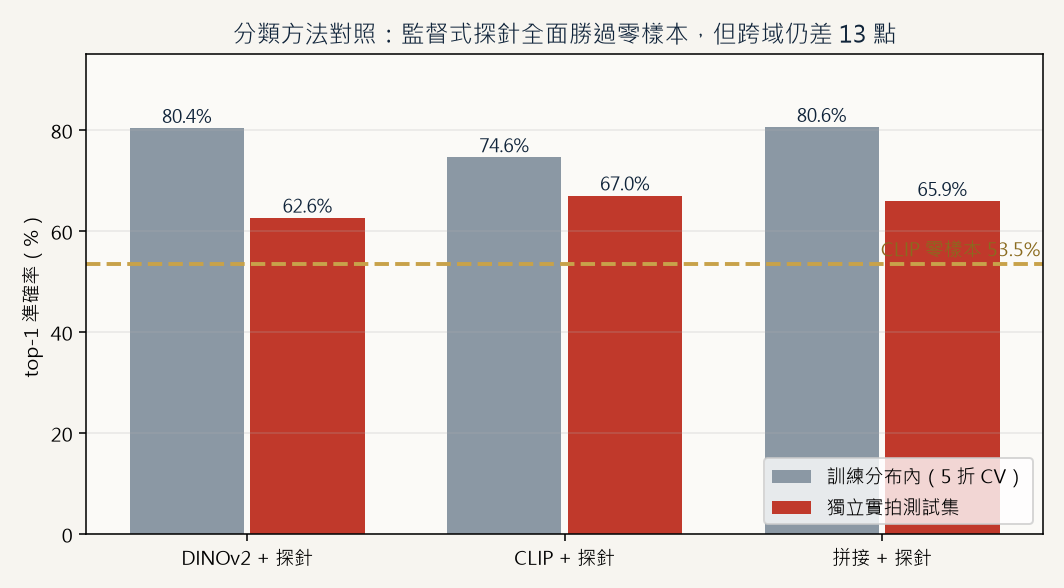
\includegraphics[width=0.78\linewidth]{figs/classifier-compare.png}
\caption{分類方法對照：監督式探針全面勝過零樣本，但跨域仍有明顯落差。}
\end{figure}

\begin{table}[H]
\centering\small
\begin{tabular}{@{}lrr@{}}
\toprule
\textbf{方法} & \textbf{訓練分布內（5 折 CV）} & \textbf{獨立實拍測試集} \\
\midrule
CLIP 零樣本 & — & 53.5\% \\
\textbf{CLIP 特徵 ＋ 探針} & 74.6\% & \textbf{67.0\%}（+13.5 點） \\
DINOv2 特徵 ＋ 探針 & \textbf{80.4\%} & 62.6\% \\
拼接（CLIP ＋ DINOv2） & 80.6\% & 65.9\% \\
\bottomrule
\end{tabular}
\caption{分類方法對照。}
\end{table}

\subsection{反直覺但重要的發現}
\textbf{DINOv2 在訓練分布內更強（80.4\% vs 74.6\%），但 CLIP 特徵跨域泛化更好（67.0\% vs 62.6\%）}——這是典型的小樣本域偏移現象：DINOv2 的細節特徵更容易過擬合訓練域。

\begin{quote}
\textbf{實務結論：任務不同就該用不同編碼器。}\\
重辨識（同一棟不同角度）$\Rightarrow$ \textbf{DINOv2}（E2 +0.143，決定性優勢）。\\
分類（小樣本、跨域）$\Rightarrow$ \textbf{CLIP 特徵 ＋ 線性探針}（67.0\%）。
\end{quote}

\noindent 主要混淆仍來自類別定義邊界：\texttt{church}$\to$\texttt{monument}（大三巴）、\texttt{civic}$\to$\texttt{casino\_hotel}。獨立實拍 67.0\% 與訓練分布內 80.4\% 之間的 13.4 點落差，\textbf{本質是資料問題（真實照片不足），不是方法問題}。

% ============================================================
\section{技術對照總表：什麼任務該用什麼}

\begin{longtable}{@{}p{3.2cm}p{3.6cm}p{3.6cm}p{4.6cm}@{}}
\toprule
\textbf{任務} & \textbf{曾用技術} & \textbf{目前採用} & \textbf{依據} \\
\midrule
\endhead
判斷是否同一棟（有 GPS） & CLIP 零樣本 & 地理先驗 ＋ DINOv2 & 90 m 先驗排除全部相似建築誤判 \\
判斷是否同一棟（無 GPS） & CLIP 零樣本 & DINOv2 ＋ SIFT/RANSAC 幾何驗證 & 內點 $\ge$15 時精確率 100\% \\
建築類型分類 & CLIP 零樣本（53.5\%） & CLIP 特徵 ＋ 線性探針（67.0\%） & 監督式探針 +13.5 點 \\
建築偵測（框） & COCO YOLO（無建築類） & 自訓 YOLO11s（11 類） & 獨立驗收偵測率 65\% \\
標註產生 & YOLO-World 自動框 & ＋ VLM 品管 ＋ 人工複核 & 找出 19\% 標註錯誤 \\
隱私處理 & OpenCV 串聯分類器（失效） & YOLO11n-face ＋ person 兩級模糊 & 實測模糊人臉 28、人物 205 \\
3D 場景重建 & 無 & （規劃中）OOOSplat 3DGS & 已能產出 \texttt{final.ply} \\
\bottomrule
\end{longtable}

% ============================================================
\section{仍未解決的問題}

\begin{enumerate}[leftmargin=1.4em,itemsep=2pt]
  \item \textbf{真實照片不足}：獨立實拍集只有 101 張、20 棟建築。分類跨域落差 13.4 點、偵測未見過建築只有 65\%，根因都是資料量。這是目前最大的瓶頸。
  \item \textbf{類別定義邊界}：大三巴牌坊（教堂遺址 vs 牌坊）、殖民地官邸（葡式 vs 公共建築）等 16.4\% 的配對屬於體系歧義，需要明確定義或合併類別。
  \item \textbf{標註仍是弱標註}：379 張的框由 YOLO-World 產生，人工尚未逐張修正。
  \item \textbf{地理先驗依賴 GPS}：室內、地下、GPS 漂移時會失準，目前只能退回純視覺並標記待複核。
  \item \textbf{DISK+LightGlue 整合失敗}：待排查 kornia 版本的 API 差異。
  \item \textbf{隱私處理未經正式評估}：只量測了模糊數量，未量測漏接率與誤模糊率。
  \item \textbf{驗證集不可比}：兩代 YOLO 的內部驗證集因重新切分而失去可比性，未來需凍結固定的外部測試集。
\end{enumerate}

% ============================================================
\section{下一步}

\begin{enumerate}[leftmargin=1.4em,itemsep=2pt]
  \item \textbf{主動學習閉環}：以現有分類器的預測機率與幾何內點數篩選「最不確定」的樣本（機率接近均勻、內點介於 5--15 的模糊帶），優先送 VLM／人工標註後重訓。預期再提升 5--10 點。
  \item \textbf{真實多視角資料（OOOSplat）}：以 3D 高斯潑濺工具環繞拍攝澳門建築，其 \texttt{work/frames/} 提供數十張\textbf{真實多視角照片}、\texttt{work/colmap/} 提供\textbf{精確相機位姿}。這同時解決三件事：補足真實照片不足、把重辨識評測從「GLB 渲染圖」升級為真實多視角、並可用位姿投影產生\textbf{幾何一致的精确標註}。
  \item \textbf{產品閾值重新校準}：依實測把併入閾值改為 DINOv2 的 0.193（幾何驗證通過時可再放寬），並加入人工複核佇列介面。
  \item \textbf{類別體系整理}：合併或明確定義 16.4\% 的歧義配對，並補抓街市、工業等少樣本類別。
\end{enumerate}

% ============================================================
\appendix
\section{完整重現指令}

\begin{verbatim}
# 階段 1-2：CLIP 基準 + 地理先驗分析
python tools/eval/render_views.py            # 7 模型 × 20 視角受控渲染（VTK 離屏）
python tools/eval/build_dataset.py           # 彙整資料集清單
python tools/eval/evaluate.py                # CLIP：AUC/ROC/閾值 + 圖表 + 報告
python tools/eval/analyze_errors.py          # 誤判來源逐對分析（路氹城案例）

# 階段 3-4：YOLO 資料管線與訓練
python tools/yolo-dataset/fetch_dataset.py --per-class 600 --subcats 2   # 抓圖（子分類遞迴 + SHA1 去重）
python tools/yolo-dataset/filter_dataset.py --restore && \
python tools/yolo-dataset/filter_dataset.py --apply --gate-exempt all   # 放寬類別關
python tools/yolo-dataset/verify_recovered.py --apply                    # 模型反向清洗
python tools/yolo-dataset/prelabel.py                                    # YOLO-World 預標註 + 分層分組切分
python tools/yolo-dataset/refine_labels.py --scan-raw --apply            # 自訓練補框
python tools/yolo-dataset/train.py --model yolo11s.pt --imgsz 768 --epochs 150 --batch 12
python tools/yolo-dataset/eval_on_cc.py                                  # 獨立照片驗收（見過/未見過）
python tools/yolo-dataset/compare_models.py                              # 同驗證集對照新舊模型

# 階段 5：VLM 品管
python tools/yolo-dataset/vlm_label.py --verify --batch 12               # DeepSeek 視覺複核
python tools/yolo-dataset/vlm_disputes.py                                # 爭議圖聯絡表（人工複核用）

# 階段 6：編碼器對照
python tools/eval/evaluate.py --encoder dino --experiments e1,e1b,e1r,e2,e4 \
       --dino-size 336 --dino-pool cls --dino-resize shortest --out-suffix=-dino-336cls
python tools/eval/compare_encoders2.py                                   # 世代對照表

# 階段 7：幾何驗證
python tools/eval/geo_verify.py --method sift                            # 檢索 + SIFT/RANSAC
python tools/eval/geo_sweep.py --method sift                             # 內點門檻掃描

# 階段 8：VLM 標註 + 線性探針
python tools/eval/probe_classifier.py --encoder clip                     # 67.0%
python tools/eval/probe_classifier.py --encoder dino --dino-size 336     # 62.6%
python tools/eval/make_history_figs.py                                   # 本報告所有圖表
\end{verbatim}

\section{核心文件清單}

\begin{longtable}{@{}p{5.4cm}p{9.6cm}@{}}
\toprule
\textbf{檔案} & \textbf{用途} \\
\midrule
\endhead
\texttt{tools/eval/evaluate.py} & 重辨識評測主程式（可切換編碼器、輸出完整報告與圖表） \\
\texttt{tools/eval/clip\_embed.py} & CLIP 編碼器封裝（含正確的類別聚合順序） \\
\texttt{tools/eval/dino\_embed.py} & DINOv2 編碼器封裝（多尺度、翻轉增強、兩種預處理） \\
\texttt{tools/eval/geo\_verify.py} & 幾何驗證（SIFT+RANSAC 與 DISK+LightGlue 兩條路） \\
\texttt{tools/eval/probe\_classifier.py} & VLM 標註 + 線性探針分類器 \\
\texttt{tools/eval/compare\_encoders2.py} & 編碼器世代對照表 \\
\texttt{tools/yolo-dataset/fetch\_dataset.py} & Commons 抓圖（子分類遞迴、SHA1 去重、授權紀錄） \\
\texttt{tools/yolo-dataset/filter\_dataset.py} & CLIP 三道清洗關卡（類別／雜物／室內） \\
\texttt{tools/yolo-dataset/prelabel.py} & YOLO-World 自動框 + 防洩漏分層分組切分 \\
\texttt{tools/yolo-dataset/refine\_labels.py} & 自訓練標註精煉（含 raw 補框） \\
\texttt{tools/yolo-dataset/verify\_recovered.py} & 以模型當裁判反向清洗 \\
\texttt{tools/yolo-dataset/vlm\_label.py} & DeepSeek 視覺品管（含類別歧義表） \\
\texttt{tools/yolo-dataset/train.py} & YOLO 訓練（暖啟動、cosine LR、增強參數） \\
\bottomrule
\end{longtable}

\end{document}
